\documentclass[11pt]{article}

\usepackage[margin=0.85in]{geometry}
\usepackage{amsmath,amssymb}
\usepackage{microtype}
\usepackage{booktabs}
\usepackage{longtable}
\usepackage[svgnames,table]{xcolor}
\usepackage{tikz}
\usetikzlibrary{
  arrows.meta,
  positioning,
  shapes.geometric,
  shapes.misc,
  fit,
  backgrounds,
  calc,
  decorations.pathreplacing,
}
\usepackage{hyperref}
\hypersetup{colorlinks=true,linkcolor=Sienna,urlcolor=SteelBlue,citecolor=Sienna}
\usepackage{url}
% \fname{long_func_name_with_underscores} renders in ttfamily and is
% allowed to break at any non-alphanumeric char (used in table cells
% where \texttt{} would overflow a fixed-width column).
\DeclareUrlCommand\fname{\urlstyle{tt}}

\setlength{\parindent}{0pt}
\setlength{\parskip}{0.55em}

%==============================================================
% Color palette
%==============================================================
\definecolor{stageOne}{HTML}{1F4E79}     % deep blue (anchor)
\definecolor{stageOneBg}{HTML}{E7EEF6}
\definecolor{stageTwo}{HTML}{0E7C7B}     % teal (Stern bump)
\definecolor{stageTwoBg}{HTML}{E0F1F1}
\definecolor{stageThree}{HTML}{6A1B9A}   % purple (grid walk)
\definecolor{stageThreeBg}{HTML}{F1E6F7}
\definecolor{newtonCore}{HTML}{B7202C}   % red core (Newton SNES)
\definecolor{newtonBg}{HTML}{FBE5E7}
\definecolor{outputCol}{HTML}{2E7D32}    % olive (output)
\definecolor{outputBg}{HTML}{E4F0E4}
\definecolor{entryCol}{HTML}{455A64}     % slate (entry/setup)
\definecolor{entryBg}{HTML}{ECEFF1}
\definecolor{fail}{HTML}{C62828}
\definecolor{success}{HTML}{2E7D32}
\definecolor{badgegray}{HTML}{616161}

%==============================================================
% TikZ styles --- every multi-line node MUST inherit align=center
%==============================================================
\tikzset{
  bigbox/.style={
    rectangle, rounded corners=6pt, line width=1.1pt, inner sep=10pt,
    align=left, font=\normalsize,
  },
  fnbox/.style={
    rectangle, rounded corners=3pt, draw=black!45, line width=0.6pt,
    fill=white, inner sep=5pt, font=\footnotesize\ttfamily,
    align=center, text width=3.2cm,    % <-- align always set
  },
  fnboxWide/.style={
    fnbox, text width=4cm,
  },
  fnboxTiny/.style={
    fnbox, text width=2.6cm, inner sep=3pt, font=\scriptsize\ttfamily,
  },
  loopbox/.style={
    rectangle, rounded corners=4pt, draw=#1, line width=0.9pt,
    fill=#1!8, inner sep=6pt, align=center, font=\small\ttfamily,
    text width=3.2cm,
  },
  decision/.style={
    diamond, draw=black!55, line width=0.7pt, fill=Cornsilk,
    inner sep=2pt, font=\footnotesize\bfseries, align=center,
    aspect=2,
  },
  badge/.style={
    rectangle, rounded corners=2pt, draw=none, fill=badgegray!18,
    text=badgegray, inner sep=2pt, font=\scriptsize\ttfamily,
  },
  arrowBig/.style={
    -{Latex[length=3mm,width=2.5mm]}, line width=1.2pt, draw=black!55,
  },
  arrowMed/.style={
    -{Latex[length=2.5mm,width=2mm]}, line width=0.9pt, draw=black!55,
  },
  arrowOK/.style={
    -{Latex[length=2.5mm,width=2mm]}, line width=0.9pt, draw=success,
  },
  arrowFail/.style={
    -{Latex[length=2.5mm,width=2mm]}, line width=0.9pt, draw=fail,
    dashed,
  },
  legend/.style={
    rectangle, draw=black!30, line width=0.4pt, fill=white,
    inner sep=4pt, font=\scriptsize, align=left,
  },
}

%==============================================================
\title{\bfseries Forward Solver Codepath\\
\large{\normalfont Visual call graph for}
\texttt{\bfseries solver\_demo\_slide15\_no\_speculative\_cs.py}}
\author{\normalsize PNPInverse / Forward solver}
\date{\today}

\begin{document}
\maketitle

\begin{abstract}\noindent
Visual call graph for the code touched when the Cs$^+$/SO$_4^{2-}$
baseline I-V demo runs --- the dataset plotted by
\texttt{plot\_solver\_demo\_slide15\_no\_speculative\_cs.py}.
Color-coded by stage:
\textcolor{stageOne}{\textbf{blue}} anchor build,
\textcolor{stageTwo}{\textbf{teal}} Stern bump,
\textcolor{stageThree}{\textbf{purple}} grid walk,
\textcolor{newtonCore}{\textbf{red}} Newton/SNES core.  Companion writeup
\emph{Derivation of the Analytic Bikerman Counterion Closure}
(\texttt{analytic\_counterion\_derivation.pdf}) covers the math behind
the Bikerman closure referenced as Layer 4.
\end{abstract}

\vspace{-0.4em}\hrule\vspace{0.4em}

%==============================================================
\section{Overview}
%==============================================================

The demo's \texttt{main()} loops over four \texttt{K0\_R4e} factors
$\{1, 10^{-6}, 10^{-12}, 10^{-18}\}$, invoking
\texttt{\_run\_one\_factor()} for each.  Each factor runs three stages
on a shared mesh:

\begin{center}
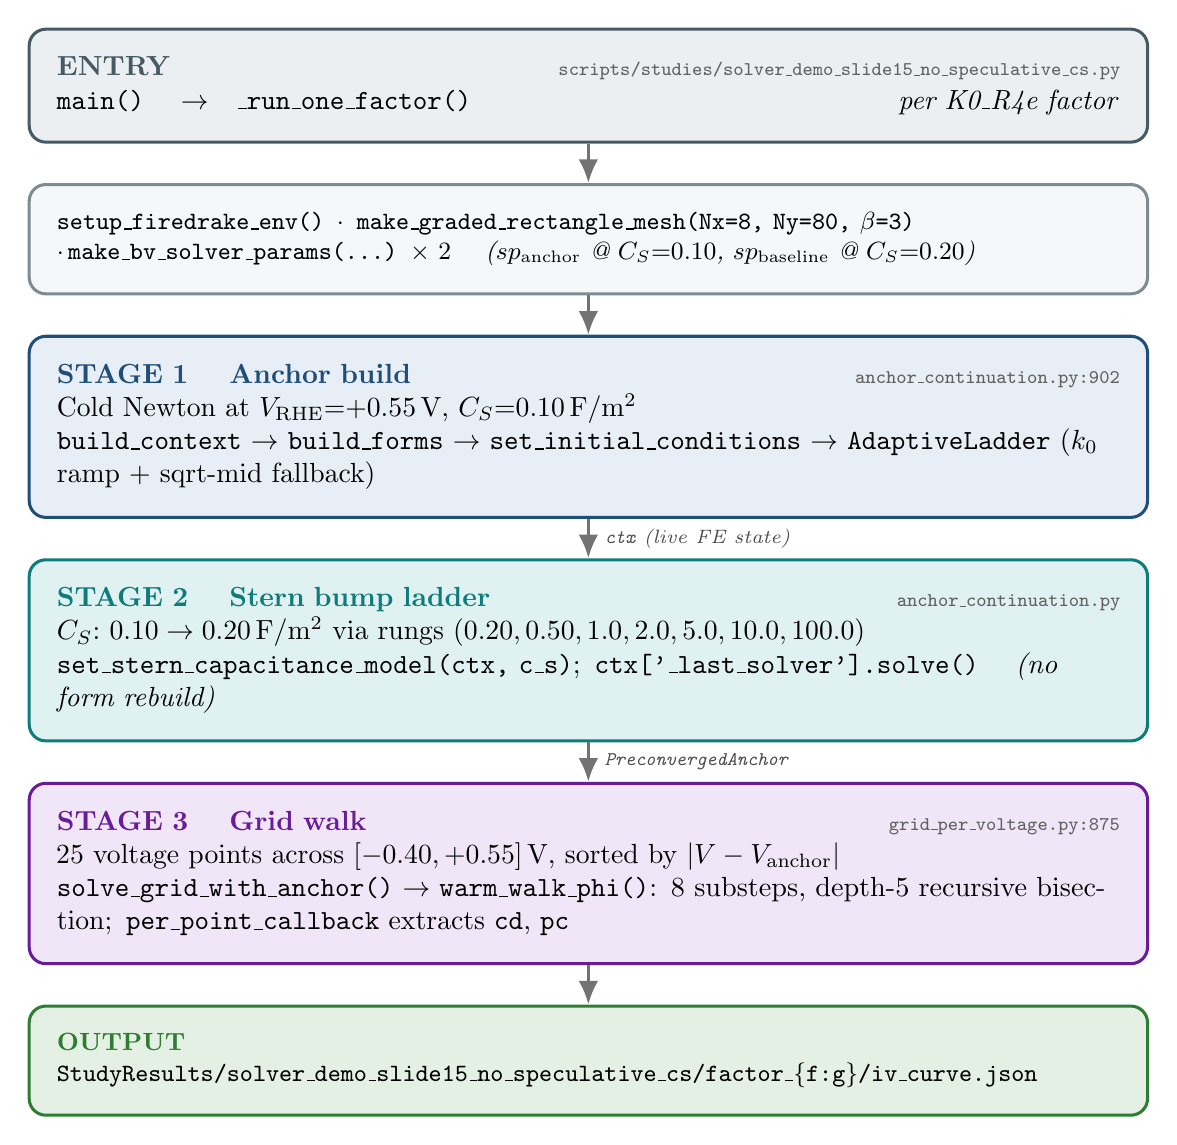
\begin{tikzpicture}[node distance=5mm]

\node[bigbox, draw=entryCol, fill=entryBg, text width=13.5cm] (entry) {%
  \textcolor{entryCol}{\textbf{ENTRY}}\hfill
  \textcolor{badgegray}{\scriptsize\ttfamily scripts/studies/solver\_demo\_slide15\_no\_speculative\_cs.py}\\
  \texttt{main()} \quad$\rightarrow$\quad \texttt{\_run\_one\_factor()}%
  \hfill\emph{per K0\_R4e factor}%
};

\node[bigbox, draw=entryCol!70, fill=entryBg!50, text width=13.5cm,
      below=of entry, font=\small] (setup) {%
  \texttt{setup\_firedrake\_env()} \,$\cdot$\,
  \texttt{make\_graded\_rectangle\_mesh(Nx=8, Ny=80, $\beta$=3)} \,$\cdot$\,%
  \texttt{make\_bv\_solver\_params(...)} $\times$ 2
  \quad\emph{($sp_{\mathrm{anchor}}$ @ $C_S{=}0.10$, $sp_{\mathrm{baseline}}$ @ $C_S{=}0.20$)}%
};

\node[bigbox, draw=stageOne, fill=stageOneBg, text width=13.5cm,
      below=of setup] (s1) {%
  \textcolor{stageOne}{\textbf{STAGE 1 \quad Anchor build}}\hfill
  \textcolor{badgegray}{\scriptsize\ttfamily anchor\_continuation.py:902}\\
  Cold Newton at $V_{\mathrm{RHE}}{=}{+}0.55$\,V, $C_S{=}0.10$\,F/m$^2$\\
  \texttt{build\_context} $\rightarrow$ \texttt{build\_forms}
    $\rightarrow$ \texttt{set\_initial\_conditions}
    $\rightarrow$ \texttt{AdaptiveLadder} ($k_0$ ramp + sqrt-mid fallback)%
};

\node[bigbox, draw=stageTwo, fill=stageTwoBg, text width=13.5cm,
      below=of s1] (s2) {%
  \textcolor{stageTwo}{\textbf{STAGE 2 \quad Stern bump ladder}}\hfill
  \textcolor{badgegray}{\scriptsize\ttfamily anchor\_continuation.py}\\
  $C_S{:}\ 0.10 \to 0.20\,\mathrm{F/m^2}$ via rungs
  $(0.20, 0.50, 1.0, 2.0, 5.0, 10.0, 100.0)$\\
  \texttt{set\_stern\_capacitance\_model(ctx, c\_s)};\,
  \texttt{ctx['\_last\_solver'].solve()}
  \quad\emph{(no form rebuild)}%
};

\node[bigbox, draw=stageThree, fill=stageThreeBg, text width=13.5cm,
      below=of s2] (s3) {%
  \textcolor{stageThree}{\textbf{STAGE 3 \quad Grid walk}}\hfill
  \textcolor{badgegray}{\scriptsize\ttfamily grid\_per\_voltage.py:875}\\
  25 voltage points across $[-0.40, +0.55]$\,V, sorted by
  $|V - V_{\mathrm{anchor}}|$\\
  \texttt{solve\_grid\_with\_anchor()} $\rightarrow$
  \texttt{warm\_walk\_phi()}: 8 substeps, depth-5 recursive bisection;
  \,\texttt{per\_point\_callback} extracts \texttt{cd}, \texttt{pc}%
};

\node[bigbox, draw=outputCol, fill=outputBg, text width=13.5cm,
      below=of s3, font=\small] (out) {%
  \textcolor{outputCol}{\textbf{OUTPUT}}\\
  \texttt{StudyResults/solver\_demo\_slide15\_no\_speculative\_cs/factor\_\{f:g\}/iv\_curve.json}%
};

\draw[arrowBig] (entry) -- (setup);
\draw[arrowBig] (setup) -- (s1);
\draw[arrowBig] (s1) -- node[right=2pt, font=\scriptsize\itshape, text=black!70]
                       {\texttt{ctx} (live FE state)} (s2);
\draw[arrowBig] (s2) -- node[right=2pt, font=\scriptsize\itshape, text=black!70]
                       {\texttt{PreconvergedAnchor}} (s3);
\draw[arrowBig] (s3) -- (out);

\end{tikzpicture}
\end{center}

%==============================================================
\section{Stage 1 --- Anchor build}
\label{sec:stage1}
%==============================================================

The first solve in any run is cold: no warm-start is available.  Stage~1
has a one-time setup (build context, build forms, install IC) followed
by a $k_0$-scale continuation loop.  Both parts must succeed for the
anchor to converge.

\subsection*{1a.\ One-time setup}

\begin{center}
\begin{tikzpicture}[node distance=4mm]

\node[fnbox, fill=stageOneBg] (bctx) {%
  \textbf{build\_context}\\\rmfamily\scriptsize dispatch.py:82\\
  \rmfamily\scriptsize\itshape mixed FE space\\
  \rmfamily\scriptsize\itshape $U$, $U_{\mathrm{prev}}$%
};

\node[fnbox, right=of bctx, fill=stageOneBg] (bfrm) {%
  \textbf{build\_forms}\\\rmfamily\scriptsize dispatch.py:89\\
  \rmfamily\scriptsize\itshape Bikerman closure\\
  \rmfamily\scriptsize\itshape $F_{\mathrm{res}}$, $J$, NLVS%
};

\node[fnbox, right=of bfrm, fill=stageOneBg] (sic) {%
  \textbf{set\_initial\_conditions}\\\rmfamily\scriptsize dispatch.py:96\\
  \rmfamily\scriptsize\itshape \texttt{debye\_boltzmann}\\
  \rmfamily\scriptsize\itshape Picard outer loop%
};

\node[loopbox=stageOne, right=of sic] (ldr) {%
  \textbf{AdaptiveLadder}\\\rmfamily\scriptsize anchor\_continuation.py:719\\
  \rmfamily\scriptsize\itshape $k_0$ continuation\\
  \rmfamily\scriptsize\itshape (\S1b below)%
};

\draw[arrowMed] (bctx) -- (bfrm);
\draw[arrowMed] (bfrm) -- (sic);
\draw[arrowMed] (sic) -- (ldr);

\end{tikzpicture}
\end{center}

Inside \texttt{build\_forms}, the Bikerman counterion machinery is
built by \texttt{build\_steric\_boltzmann\_expressions} and
\texttt{add\_boltzmann\_counterion\_residual} in
\texttt{boltzmann.py}.  Inside \texttt{set\_initial\_conditions},
\texttt{picard\_outer\_loop\_general} in \texttt{picard\_ic.py} runs a
$2 \times 2$ scalar Picard on $(\psi_S, \psi_D)$ to seed the EDL.

\subsection*{1b.\ Continuation loop (AdaptiveLadder)}

The loop ramps the kinetic prefactor $k_0$ from $10^{-12}$ (kinetics
effectively off, diffusion-only Newton) up to the production value.
On each rung it does a steady-state solve; on success it advances; on
failure it inserts the geometric midpoint and retries:

\begin{center}
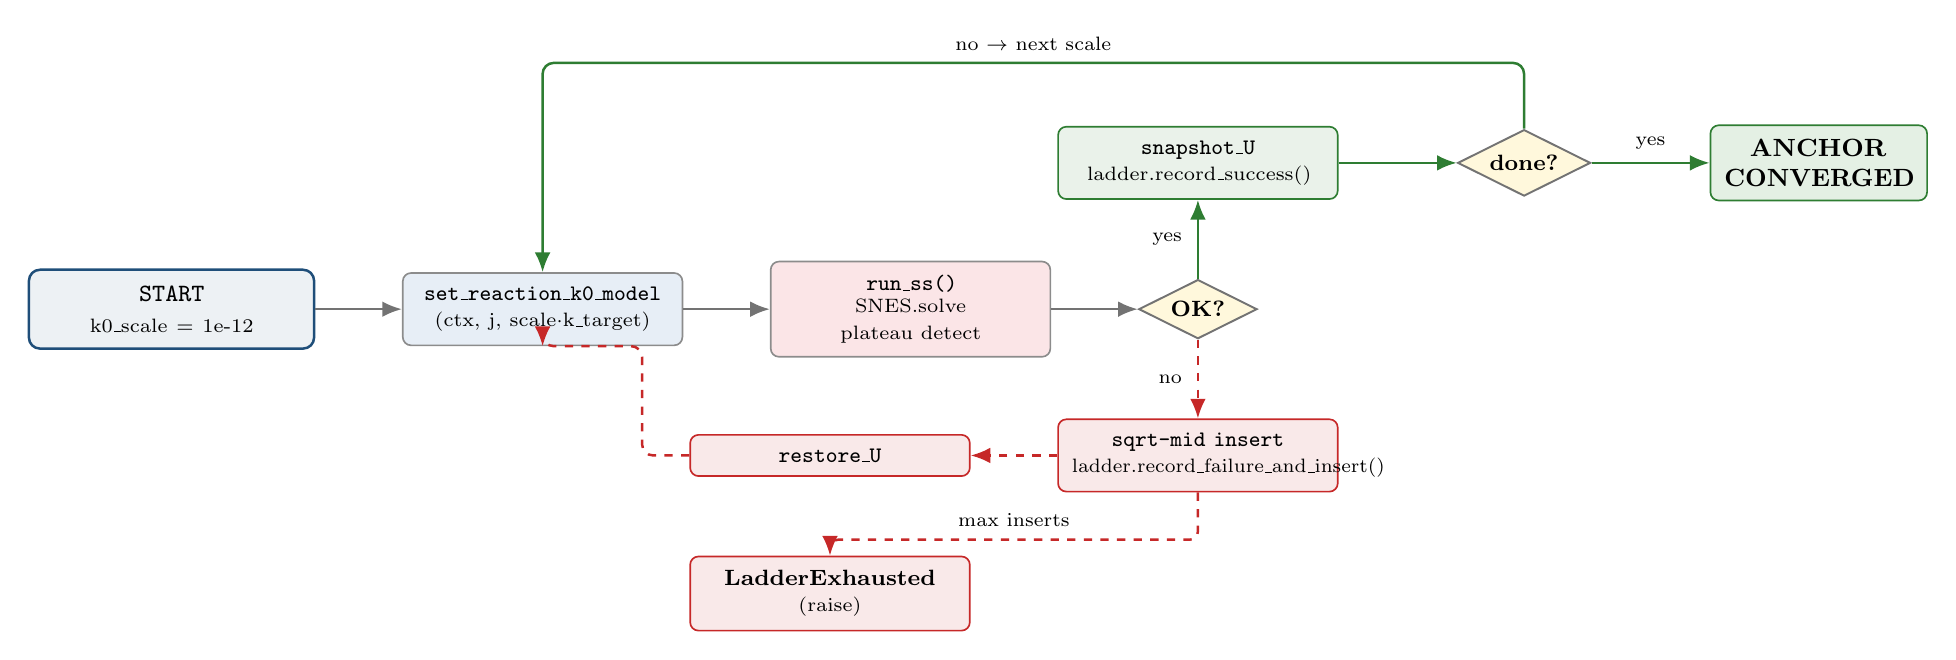
\begin{tikzpicture}[node distance=7mm and 11mm]

\node[loopbox=stageOne] (start) {%
  \textbf{START}\\\rmfamily\scriptsize k0\_scale = 1e-12%
};
\node[fnbox, right=of start, fill=stageOneBg] (setk) {%
  set\_reaction\_k0\_model\\\rmfamily\scriptsize (ctx, j, scale$\cdot$k\_target)%
};
\node[fnbox, right=of setk, fill=newtonBg] (runss2) {%
  \textbf{run\_ss()}\\\rmfamily\scriptsize SNES.solve\\\rmfamily\scriptsize plateau detect%
};
\node[decision, right=of runss2] (ok) {OK?};

\node[fnbox, above=10mm of ok, fill=success!10, draw=success] (snap) {%
  \textbf{snapshot\_U}\\\rmfamily\scriptsize ladder.record\_success()%
};
\node[fnbox, below=10mm of ok, fill=fail!10, draw=fail] (insert) {%
  \textbf{sqrt-mid insert}\\\rmfamily\scriptsize ladder.record\_failure\_and\_insert()%
};
\node[fnbox, left=of insert, fill=fail!10, draw=fail] (restore) {%
  \textbf{restore\_U}%
};

\node[decision, right=15mm of snap] (done) {done?};
\node[fnbox, right=15mm of done, fill=outputBg, draw=outputCol,
      text width=2.4cm, font=\small] (anchOk) {%
  \textbf{ANCHOR}\\\textbf{CONVERGED}%
};
\node[fnbox, below=10mm of restore, fill=fail!10, draw=fail,
      font=\footnotesize] (exhausted) {%
  \textbf{LadderExhausted}\\\rmfamily\scriptsize (raise)%
};

% Flow arrows
\draw[arrowMed] (start) -- (setk);
\draw[arrowMed] (setk)  -- (runss2);
\draw[arrowMed] (runss2)-- (ok);

\draw[arrowOK]   (ok.north) -- node[left=2pt, font=\scriptsize] {yes} (snap.south);
\draw[arrowFail] (ok.south) -- node[left=2pt, font=\scriptsize] {no}  (insert.north);

\draw[arrowFail] (insert) -- (restore);

% restore -> setk loop-back (down, left, up, right into setk.south)
\coordinate (rLoopA) at ($(restore.west) + (-0.6, 0)$);
\coordinate (rLoopB) at (rLoopA |- setk.south);
\coordinate (rLoopC) at (setk.south |- rLoopB);
\draw[arrowFail, rounded corners=4pt]
   (restore.west) -- (rLoopA) -- (rLoopB) -- (rLoopC) -- (setk.south);

% insert -> exhausted (down then around)
\draw[arrowFail, rounded corners=3pt]
   (insert.south) -- ($(insert.south) + (0, -0.6)$) -| (exhausted.north)
   node[pos=0.25, above=1pt, font=\scriptsize] {max inserts};

\draw[arrowOK] (snap) -- (done);
\draw[arrowOK] (done.east) -- node[above=1pt, font=\scriptsize] {yes} (anchOk);

% done -> setk loop-back (up, over the top, down into setk.north)
\coordinate (topRow) at ($(snap.north) + (0, 0.8)$);
\coordinate (doneTop) at (done.north |- topRow);
\coordinate (setkTop) at (setk.north |- topRow);
\draw[arrowOK, rounded corners=4pt]
   (done.north) -- (doneTop) -- (setkTop) -- (setk.north);
\node[above=1pt, font=\scriptsize]
   at ($(doneTop)!0.5!(setkTop)$) {no $\rightarrow$ next scale};

\end{tikzpicture}
\end{center}

After \texttt{max\_inserts\_per\_step=4} consecutive failures, the
loop raises \texttt{LadderExhausted}.

%==============================================================
\section{Stage 2 --- Stern bump ladder}
%==============================================================

$C_S = 0.20$\,F/m$^2$ won't converge cold, but $C_S = 0.10$ does.
After Stage 1 lands at $C_S = 0.10$, ramp $C_S$ upward through a
verified rung sequence.  Each rung mutates a shared FE
\texttt{Constant} on \texttt{ctx} (no form rebuild) and reuses Stage 1's
solver:

\begin{center}
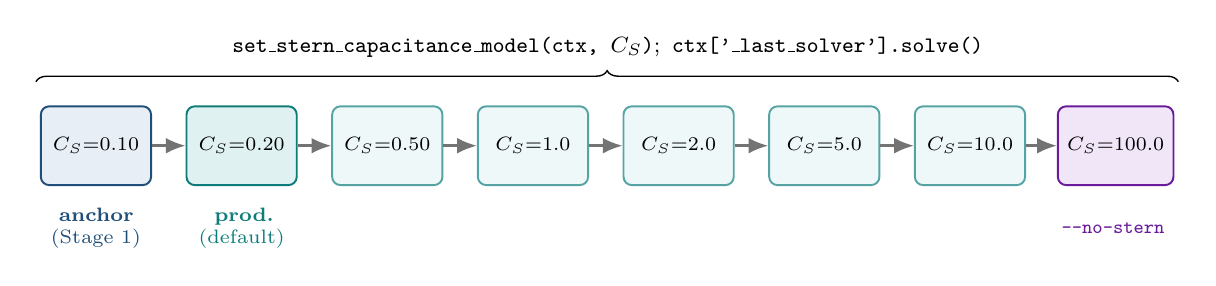
\begin{tikzpicture}[every node/.style={align=center}]

\foreach \i/\val/\dcol/\fcol in {%
  0/0.10/stageOne/stageOneBg,%
  1/0.20/stageTwo/stageTwoBg,%
  2/0.50/stageTwo!70/stageTwoBg!50,%
  3/1.0/stageTwo!70/stageTwoBg!50,%
  4/2.0/stageTwo!70/stageTwoBg!50,%
  5/5.0/stageTwo!70/stageTwoBg!50,%
  6/10.0/stageTwo!70/stageTwoBg!50,%
  7/100.0/stageThree/stageThreeBg%
}
{
  \pgfmathsetmacro{\xshift}{\i*1.85}
  \node[draw=\dcol, fill=\fcol, rounded corners=3pt, line width=0.7pt,
        minimum width=1.4cm, minimum height=1cm, align=center,
        font=\scriptsize]
   (r\i) at (\xshift, 0) {$C_S{=}$\val};
}

\node[font=\scriptsize, text=stageOne, align=center, text width=1.5cm] at (0, -1.05)
   {\textbf{anchor}\\\rmfamily(Stage 1)};
\node[font=\scriptsize, text=stageTwo, align=center, text width=1.5cm] at (1.85, -1.05)
   {\textbf{prod.}\\\rmfamily(default)};
\node[font=\scriptsize, text=stageThree, align=center, text width=1.6cm] at (12.95, -1.05)
   {\textbf{\texttt{--no-stern}}};

\foreach \i/\j in {0/1, 1/2, 2/3, 3/4, 4/5, 5/6, 6/7}
  \draw[arrowMed] (r\i) -- (r\j);

\draw [decorate, decoration={brace, amplitude=4pt}, line width=0.5pt]
  ($(r0.north west) + (-0.05, 3mm)$) -- ($(r7.north east) + (0.05, 3mm)$);
\node[font=\footnotesize, anchor=south] at (6.5, 1.0)
  {\texttt{set\_stern\_capacitance\_model(ctx, $C_S$)};\,
   \texttt{ctx['\_last\_solver'].solve()}};

\end{tikzpicture}
\end{center}

The bump-ladder helper truncates the verified rung list at the first
rung $\geq$ target, so a $C_S = 0.20$ run lands in two steps and the
no-Stern run uses all seven.

%==============================================================
\section{Stage 3 --- Grid walk}
%==============================================================

The grid walk visits 25 voltage points sorted by distance from the
anchor.  Each point gets a fresh FE context built at its own
$V_{\mathrm{RHE}}$ and is warm-started from its nearest
already-converged neighbor.  Voltage gaps are bridged by
\texttt{warm\_walk\_phi}, which substeps and recursively bisects on
failure.

\subsection*{3a.\ Grid layout and Frumkin cliff}

\begin{center}
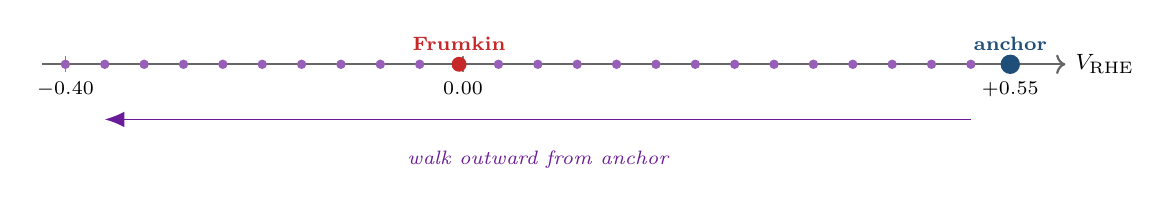
\begin{tikzpicture}

\draw[->, line width=0.8pt, draw=black!60] (-0.3, 0) -- (12.7, 0)
  node[right, font=\footnotesize] {$V_{\mathrm{RHE}}$};

% tick labels
\draw[draw=black!50] (0, 0.1) -- (0, -0.1) node[below, font=\scriptsize] {$-0.40$};
\draw[draw=black!50] (5.05, 0.1) -- (5.05, -0.1) node[below, font=\scriptsize] {$0.00$};
\draw[draw=black!50] (12, 0.1) -- (12, -0.1) node[below, font=\scriptsize] {$+0.55$};

% 25 grid points: linspace(-0.40, 0.55, 25) maps to x in [0, 12]
\foreach \i in {0,1,...,24}
{
  \pgfmathsetmacro{\xpos}{\i * 0.5}
  \pgfmathtruncatemacro{\isAnchor}{\i==24 ? 1 : 0}
  \pgfmathtruncatemacro{\isCliff}{\i==10 ? 1 : 0}
  \ifnum\isAnchor=1
    \fill[stageOne] (\xpos, 0) circle (3.5pt);
    \node[above=1.5pt, font=\scriptsize, text=stageOne]
      at (\xpos, 0) {\textbf{anchor}};
  \else
    \ifnum\isCliff=1
      \fill[fail] (\xpos, 0) circle (2.7pt);
      \node[above=1.5pt, font=\scriptsize, text=fail]
        at (\xpos, 0) {\textbf{Frumkin}};
    \else
      \fill[stageThree!70] (\xpos, 0) circle (1.7pt);
    \fi
  \fi
}

% Walk-direction annotation
\draw[arrowMed, draw=stageThree, line width=0.6pt]
  (11.5, -0.7) -- (0.5, -0.7);
\node[below=8pt, font=\scriptsize\itshape, text=stageThree]
  at (6, -0.7) {walk outward from anchor};

\end{tikzpicture}
\end{center}

The red dot at $V \approx 0$\,V is the Frumkin cliff --- the voltage
where Bikerman SO$_4^{2-}$ saturation suddenly clamps the diffuse-layer
charge balance.  The walk visits the 24 non-anchor points in order of
increasing $|V - V_{\mathrm{anchor}}|$, so anything past the cliff is
warm-started from a neighbor still on the anodic side.

\subsection*{3b.\ One warm-walk step --- substeps and recursive bisection}

Between two consecutive visited points the walk substeps in 8 even
increments; if Newton fails at any substep, the failing interval is
halved and the walk recurses, up to depth 5 ($32\times$ refinement):

\begin{center}
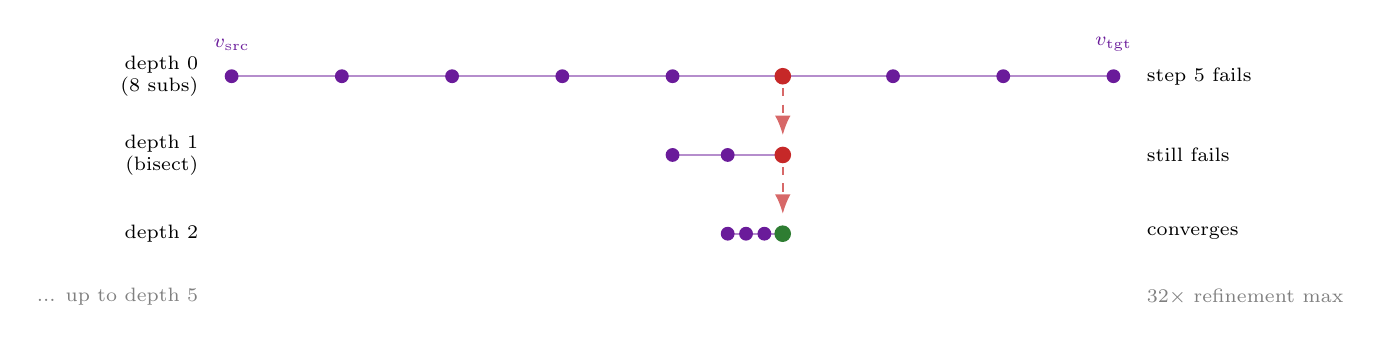
\begin{tikzpicture}

% Row labels
\node[anchor=east, font=\scriptsize, align=right] at (-0.3, 3.0)
   {depth 0\\(8 subs)};
\node[anchor=east, font=\scriptsize, align=right] at (-0.3, 2.0)
   {depth 1\\(bisect)};
\node[anchor=east, font=\scriptsize, align=right] at (-0.3, 1.0)
   {depth 2};
\node[anchor=east, font=\scriptsize, text=black!50, align=right]
   at (-0.3, 0.2) {... up to depth 5};

% Depth 0: 8 substeps spanning [0, 11.2]; step 5 fails
\draw[draw=stageThree!50, line width=0.6pt] (0, 3.0) -- (11.2, 3.0);
\foreach \i in {0,1,...,8}
{
  \pgfmathsetmacro{\xpos}{\i * 1.4}
  \pgfmathtruncatemacro{\isFail}{\i==5 ? 1 : 0}
  \ifnum\isFail=1
    \fill[fail] (\xpos, 3.0) circle (3pt);
  \else
    \fill[stageThree] (\xpos, 3.0) circle (2.5pt);
  \fi
}
\node[anchor=west, font=\scriptsize] at (11.5, 3.0) {step 5 fails};
\node[anchor=south, font=\scriptsize, text=stageThree]
   at (0, 3.2) {$v_{\mathrm{src}}$};
\node[anchor=south, font=\scriptsize, text=stageThree]
   at (11.2, 3.2) {$v_{\mathrm{tgt}}$};

% Bisection arrow from depth 0 step 5 down to depth 1
\draw[arrowFail, draw=fail!70] (7.0, 2.85) -- (7.0, 2.25);

% Depth 1: 3 points between step 4 and step 5; last fails
\draw[draw=stageThree!50, line width=0.6pt] (5.6, 2.0) -- (7.0, 2.0);
\foreach \i in {0,1,2}
{
  \pgfmathsetmacro{\xpos}{5.6 + \i * 0.7}
  \pgfmathtruncatemacro{\isFail}{\i==2 ? 1 : 0}
  \ifnum\isFail=1
    \fill[fail] (\xpos, 2.0) circle (3pt);
  \else
    \fill[stageThree] (\xpos, 2.0) circle (2.5pt);
  \fi
}
\node[anchor=west, font=\scriptsize] at (11.5, 2.0) {still fails};

% Bisection arrow from depth 1 down to depth 2
\draw[arrowFail, draw=fail!70] (7.0, 1.85) -- (7.0, 1.25);

% Depth 2: 4 points; converges
\draw[draw=stageThree!50, line width=0.6pt] (6.3, 1.0) -- (7.0, 1.0);
\foreach \i in {0,1,2,3}
{
  \pgfmathsetmacro{\xpos}{6.3 + \i * 0.233}
  \pgfmathtruncatemacro{\isOK}{\i==3 ? 1 : 0}
  \ifnum\isOK=1
    \fill[success] (\xpos, 1.0) circle (3pt);
  \else
    \fill[stageThree] (\xpos, 1.0) circle (2.5pt);
  \fi
}
\node[anchor=west, font=\scriptsize] at (11.5, 1.0) {converges};

\node[anchor=west, font=\scriptsize, text=black!50] at (11.5, 0.2)
   {$32\times$ refinement max};

\end{tikzpicture}
\end{center}

\begin{center}\footnotesize
\tikz[baseline=-0.6ex]{\fill[stageOne] (0,0) circle (3pt);}\,\,anchor \quad
\tikz[baseline=-0.6ex]{\fill[stageThree] (0,0) circle (2.5pt);}\,\,grid pt / substep \quad
\tikz[baseline=-0.6ex]{\fill[success] (0,0) circle (3pt);}\,\,converges after bisection \quad
\tikz[baseline=-0.6ex]{\fill[fail] (0,0) circle (3pt);}\,\,SNES diverges
\end{center}

The Frumkin cliff at $V \approx 0$\,V is exactly where this recursive
bisection earns its keep: substepping alone often isn't fine enough,
and without depth-5 recursion the walk would mark several anodic-side
points unconvergeable.

%==============================================================
\section{Layered defense --- what keeps Newton in basin}
%==============================================================

The solver is defense in depth.  Each layer below is one form of
preconditioning around the innermost Newton/SNES solve --- outer
layers either reduce the residual the inner solve must handle, or
recover when the inner solve fails.

\begin{center}
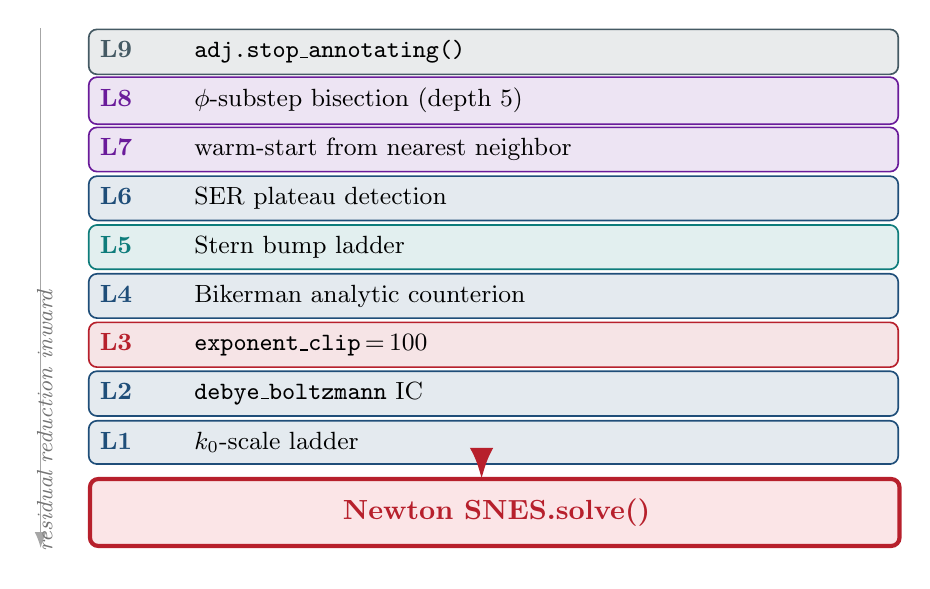
\begin{tikzpicture}

\foreach \layer/\col/\desc/\y [count=\i] in {%
  L9/entryCol/{\texttt{adj.stop\_annotating()}}/0,%
  L8/stageThree/{$\phi$-substep bisection (depth 5)}/-0.62,%
  L7/stageThree/{warm-start from nearest neighbor}/-1.24,%
  L6/stageOne/{SER plateau detection}/-1.86,%
  L5/stageTwo/{Stern bump ladder}/-2.48,%
  L4/stageOne/{Bikerman analytic counterion}/-3.10,%
  L3/newtonCore/{\texttt{exponent\_clip}\,=\,100}/-3.72,%
  L2/stageOne/{\texttt{debye\_boltzmann} IC}/-4.34,%
  L1/stageOne/{$k_0$-scale ladder}/-4.96%
}
{
  \node[draw=\col, fill=\col!12, rounded corners=3pt,
        text width=10cm, minimum height=0.55cm,
        inner sep=4pt, anchor=west, line width=0.6pt,
        align=left, font=\small]
   at (0, \y) {%
     \makebox[1.2cm][l]{\textbf{\textcolor{\col}{\layer}}}\desc%
   };
}

% Newton core at bottom (more prominent)
\node[draw=newtonCore, fill=newtonBg, rounded corners=3pt,
      text width=10cm, minimum height=0.85cm,
      inner sep=4pt, anchor=west, font=\bfseries, align=center,
      line width=1.5pt]
  at (0, -5.85) {%
    \textcolor{newtonCore}{Newton SNES.solve()}%
};

% Down-arrow connecting L1 to Newton core — larger and red
\draw[-{Latex[length=4mm,width=3mm]}, line width=1.8pt, draw=newtonCore]
   (5, -5.23) -- (5, -5.43);

% Left side label
\draw[draw=black!35, line width=0.4pt, -{Latex[length=2mm]}]
  (-0.6, 0.3) -- (-0.6, -6.3);
\node[anchor=east, rotate=90, font=\footnotesize\itshape, text=black!55]
  at (-0.55, -2.9) {residual reduction inward};

\end{tikzpicture}
\end{center}

{\footnotesize
\renewcommand{\arraystretch}{1.2}
\begin{longtable}{@{}>{\raggedright\arraybackslash}p{0.40cm}%
                    >{\raggedright\arraybackslash}p{2.8cm}%
                    >{\raggedright\arraybackslash}p{4.6cm}%
                    >{\raggedright\arraybackslash}p{4.8cm}@{}}
\toprule
\textbf{L} & \textbf{Mechanism} & \textbf{Location} & \textbf{Why it matters} \\
\midrule
\endhead

1 & $k_0$-scale ladder ($10^{-12} \to 1.0$) &
  \fname{AdaptiveLadder} @ \fname{anchor_continuation.py:719} &
  Starts with kinetics off (Newton sees a diffusion-only problem),
  ramps to production $k_0$.  Sqrt-midpoint insertion recovers from
  failed rungs without restart. \\
\addlinespace
2 & \fname{debye_boltzmann} IC &
  \fname{picard_ic.py} $\to$ \fname{set_ic_debye_boltzmann_logc_muh} &
  Seeds the EDL with the right composite $\psi_S + \psi_D$ structure
  so Newton's initial residual is $\mathcal{O}(1)$ rather than
  $\mathcal{O}(10^{26})$. \\
\addlinespace
3 & \fname{exponent_clip}\,=\,100 &
  \fname{forms_logc_muh.py:_build_eta_clipped} &
  Clamps $\eta_{\mathrm{scaled}}$ before the $\alpha \cdot n_e$
  multiplication.  Without it $\exp(\alpha n_e \eta)$ over/underflows
  and SNES gets \texttt{Inf} in $F$. \\
\addlinespace
4 & Bikerman analytic counterion &
  \fname{boltzmann.py:build_steric_boltzmann_expressions} &
  Cs$^+$ and SO$_4^{2-}$ never enter the Newton state vector --- they
  are closed-form functionals of $\phi$.  Eliminates transport modes
  that would otherwise stall Newton in the Debye layer. \\
\addlinespace
5 & Stern bump ladder &
  demo \fname{_stern_bump_ladder} $+$
  \fname{set_stern_capacitance_model} &
  $C_S = 0.20$ won't anchor cold; $C_S = 0.10$ will.  Build at $0.10$,
  ramp to $0.20$ via verified rungs without form rebuild. \\
\addlinespace
6 & SER plateau detection &
  \fname{make_run_ss} @ \fname{grid_per_voltage.py:135} &
  Newton alone doesn't tell you BV is steady --- you need $\int j\,ds$
  to stop drifting.  Plateau detector watches the surface flux and
  declares success when it stops moving. \\
\addlinespace
7 & Warm-start from nearest neighbor &
  \fname{solve_grid_with_anchor} @ \fname{grid_per_voltage.py:875} &
  Newton's basin radius in $\phi_{\mathrm{applied}}$ is
  $\sim 0.05$\,V; the anchor is up to $0.95$\,V from the cathodic
  edge, so the walk visits points in distance order, not list order. \\
\addlinespace
8 & Recursive $\phi$-substep bisection &
  \fname{warm_walk_phi} @ \fname{grid_per_voltage.py:218} &
  If the 8-substep warm walk fails between two grid points, the
  failing interval is halved and retried up to depth 5
  ($32\times$ refinement).  Catches the Frumkin cliff at
  $V \approx 0$\,V. \\
\addlinespace
9 & \fname{adj.stop_annotating()} &
  demo script around solver calls &
  Forward demo doesn't need the adjoint tape; wrapping prevents
  pyadjoint from recording $10^4{+}$ ops per solve, which would
  OOM the process. \\

\bottomrule
\end{longtable}
}% end \footnotesize for longtable

%==============================================================
\section{Files touched, by stage}
%==============================================================

\paragraph{\textcolor{stageOne}{Stage 1 --- anchor build}}
\begin{itemize}\setlength{\itemsep}{1pt}\small
\item \texttt{anchor\_continuation.py}:
  \texttt{solve\_anchor\_with\_continuation},
  \texttt{AdaptiveLadder},
  \texttt{solve\_reaction\_k0\_model}
\item \texttt{dispatch.py}:
  \texttt{build\_context},
  \texttt{build\_forms},
  \texttt{set\_initial\_conditions}
\item \texttt{forms\_logc\_muh.py}:
  \texttt{build\_context\_logc\_muh},
  \texttt{build\_forms\_logc\_muh},
  \texttt{set\_ic\_debye\_boltzmann\_logc\_muh},
  \texttt{\_build\_eta\_clipped}
\item \texttt{boltzmann.py}:
  \texttt{build\_steric\_boltzmann\_expressions},
  \texttt{add\_boltzmann\_counterion\_residual}
\item \texttt{picard\_ic.py},
  \texttt{multi\_ion.py},
  \texttt{mesh.py},
  \texttt{nondim.py}
\end{itemize}

\paragraph{\textcolor{stageTwo}{Stage 2 --- Stern bump}}
\begin{itemize}\setlength{\itemsep}{1pt}\small
\item \texttt{anchor\_continuation.py}:
  \texttt{set\_stern\_capacitance\_model} (reuses Stage 1's
  \texttt{NonlinearVariationalSolver} stored on \texttt{ctx})
\end{itemize}

\paragraph{\textcolor{stageThree}{Stage 3 --- grid walk}}
\begin{itemize}\setlength{\itemsep}{1pt}\small
\item \texttt{grid\_per\_voltage.py}:
  \texttt{solve\_grid\_with\_anchor},
  \texttt{warm\_walk\_phi},
  \texttt{\_march} (bisection),
  \texttt{snapshot\_U}, \texttt{restore\_U},
  \texttt{make\_run\_ss}
\item \texttt{observables.py}:
  \texttt{\_build\_bv\_observable\_form}
\item \texttt{dispatch.py}: same
  \texttt{build\_context} / \texttt{build\_forms} /
  \texttt{set\_initial\_conditions} as Stage 1, but invoked once
  per voltage on a fresh \texttt{ctx}
\end{itemize}

%==============================================================
\section{Per-factor wall time (typical)}
%==============================================================

\begin{center}
\renewcommand{\arraystretch}{1.15}
\begin{tabular}{@{}lr l@{}}
\toprule
\textbf{Stage} & \textbf{Wall time} & \textbf{Dominant cost} \\
\midrule
Stage 1 anchor build      & 20--60\,s   &
   $\sim$5 ladder rungs $\times$ several SS steps $\times$ Newton \\
Stage 2 Stern bump        & 10--30\,s   &
   7 rungs $\times$ 1 Newton solve each \\
Stage 3 grid walk         & 2--5\,min   &
   25 pts $\times$ warm-walk $\times$ $\sim$8 substeps $\times$ Newton \\
\midrule
\textbf{Total / factor}   & \textbf{3--7\,min}    & \\
\textbf{4-factor sweep}   & \textbf{15--30\,min}  & \\
\bottomrule
\end{tabular}
\end{center}

Stage 3 dominates wall time; the Frumkin cliff near $V \approx 0$\,V
is the main source of variance because it triggers bisection events.

%==============================================================
\section*{Notes}
%==============================================================

\begin{itemize}
\setlength{\itemsep}{2pt}
\item The plot script
  \texttt{plot\_solver\_demo\_slide15\_no\_speculative\_cs.py} reads
  only the JSON files this codepath writes --- no solver code is
  exercised by plotting.
\item The same call graph holds for the no-Stern variant
  (\texttt{-{}-no-stern}); the only differences are
  \texttt{stern\_final}\,=\,100.0 and the bump ladder reaching the
  rightmost (purple) rung in the Stage~2 diagram.
\item This is \emph{not} the inverse-solver codepath.  The inverse
  path (\texttt{scripts/Inference/}) is paused and uses different
  orchestrators (\texttt{Inference/lm\_tikhonov.py}, etc.).
\item The Bikerman closure (Layer 4) is derived in detail in the
  companion writeup
  \emph{Derivation of the Analytic Bikerman Counterion Closure}
  (\texttt{analytic\_counterion\_derivation.pdf}, this directory).
\end{itemize}

\end{document}
